
All references in the following section will be refering to the code listed in Appendix~\ref{app:Code}.

There are three big parts. The first is a solver, 
which solves a FEM-problem, using a certain number of cells, and a certain degree of polynomials. 
The second is a function which calculates the error in $L_2$,
which comes directly from~\cite{"fen-tutorial"}. 
The last part is two functions, which loop over 
various numbers of cells and polynomial degrees, 
and outputs a table. 

We start on line 10 by defining our solution $u$ as the function from Equation~\eqref{eq:app_dirichlet},
after which we define two different interpolations of $u$ using the packages "numpy" and "ufl". 
We do this for convience, as numpy are better for numerical apporiximations, and ufl is 
easier to work with in FEniCSx.
Next, we need to define the mesh and the function space we will be working in. 
We do this on line 16-22, where $N$ defines the number of cells in each directions of our mesh, resulting in $N^2$ elements in total.
Then `degree' defines the degree of polynomials we use in each cell.
Next step in the process is to define the space of trial functions 
and the space of test functions, which we do on line 24-26.
In a different situation, these two spaces could have been different.

We then define the boundary condition, which is simply the function $k$, as mentioned earlier.
With the boundary condition established we can move on to defining the bilinear form $a$ and the linear form $L$.
With all this in place, we can now solve the problem using the PETSc interface from FEniCSx. 
\begin{figure}[H]
    \centering
    \begin{subfigure}{.3\textwidth}
        \centering
        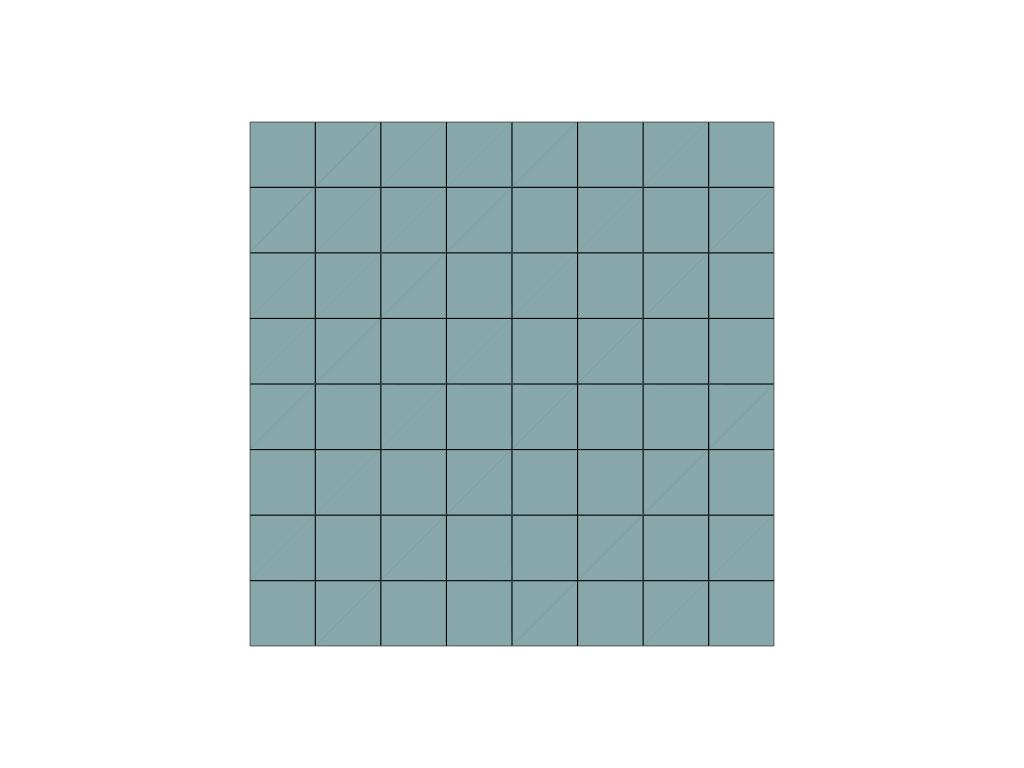
\includegraphics[width=\textwidth]{Afsnit/Application/figurer/screenshot_1.jpeg}
        \caption{Quadrilaterial slicing of domain}~\label{fig:FEM_plot_domain}
      \end{subfigure}
    \begin{subfigure}{.3\textwidth}
        \centering
        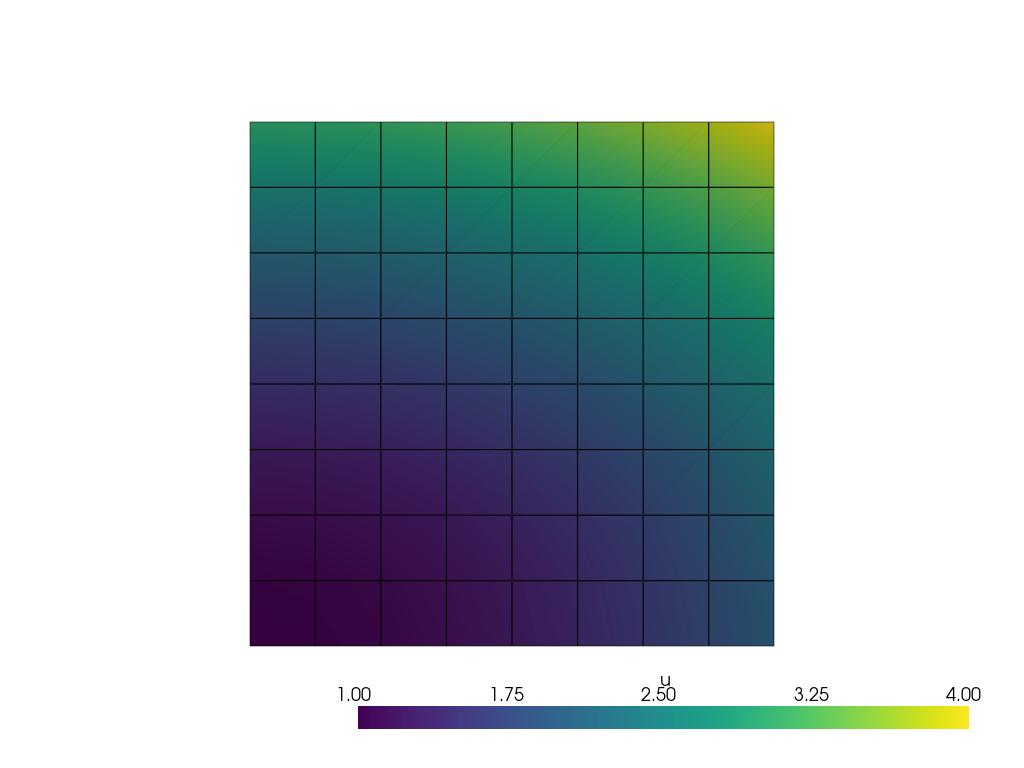
\includegraphics[width=\textwidth]{Afsnit/Application/figurer/screenshot_2.jpeg}
        \caption{Domain colored in accordance to the warping scalar obtained by the solution $u_h$ ranging from 1 to 4}~\label{fig:FEM_plot_warped_domain}
    \end{subfigure}
    \begin{subfigure}{.3\textwidth}
        \centering
        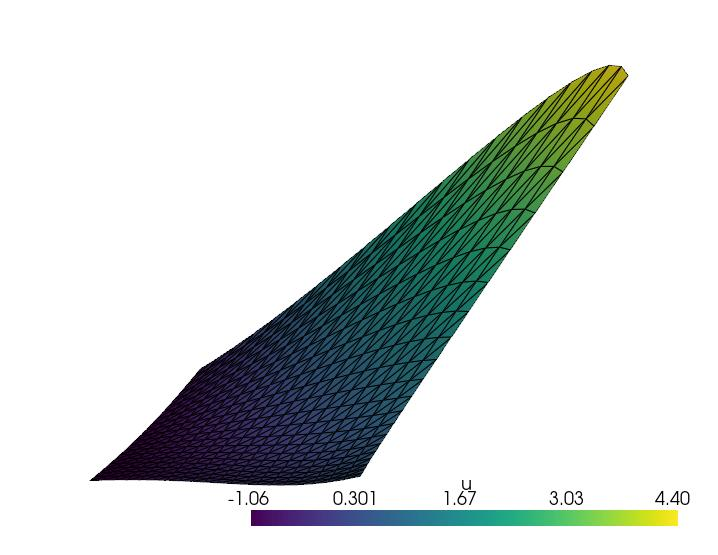
\includegraphics[width=\textwidth]{Afsnit/Application/figurer/screenshot_3.jpeg}
        \caption{The same domain warped with respect to the scalar value, ranging from 1 to 4}~\label{fig:FEM_plot_3D}
    \end{subfigure}
    \caption{Plots of the ?quadrilaterialerised? domain}~\label{fig:FEM_plots}
\end{figure}

As discussed earlier the first step in approximatin the solution to a partial differential equation is do establish a fitting domain. In our example we have chosen a square ranging from $(-1,-1)$ to $(1,1)$.
The domain is then quadrilaterialerised or triangulised depending on the specific scenario, in Plot~\ref{fig:FEM_plot_domain} we have chosen to slice the domain into quadrilaterials, of equal size making the domain regular.
After the domain is sliced and we have estimated the soltion using the nodal points obtained in the quadrilaterials, we can plot the solution over the domain to obtain Plot~\refeq{fig:FEM_plot_warped_domain} where each cell is colored in accordance to the value in the given point.
We can then warp the domain to give a clear look on what exactly our solution looks like in 3D, this is shown in Plot~\refeq{fig:FEM_plot_3D}, where it is also obvious what the visual meaning of a boundary condition, since it is clear the boundary follows the specificied function $1 + x_0^2 + 2x_1^2$.
%The convergence rate tells us how fast the error decreases as we increase the number of elements in our mesh.
%Ideally we would like the error to decrease as we decrease the mesh size. This corresponds to showing that the error $e=k_e-k_h$ is bounded by $\|e\|\leq Ch^r$, 
%with being the mesh size, $r$ the convergence rate and $C$ some constant independent of $h$.

Examining the error can show us the 
convergence rate, which tells us how fast the error decreases as we increase the number of elements in our mesh and degree of polynomials.
We will show this imperically by computing the error for different mesh sizes and degrees and comparing them. 
In Table~\ref{tab:convergence_l2}, 
the error for five different mesh sizes are shown. 
For each different mesh, the solution have been approximated using polynomials of degree one through ten.
%The table shows the error decreases as we decrease the cell size for all degrees of the polynomials, 
%and smaller sizes of cells increases the convergence rate dramatically. 
%For example, at $h=0.03125$, the error is less than $40$ already at degree $6$, and 
%for $h=0.0625$ to reach the same error, we need a degree of $8$, while bigger cells do not 
%even reach that size of error.
%Besides that, we can observe for a polynomial of degree $10$ the error changes by a factor $10^{-9}$ from a 
%cell size of $0.25$ to $0.015625$. Meanwhile, for a polynomial of degree $5$ the error changes by a 
%factor $10^{-6}$, and for a polynomial of degree $1$ the error changes by a factor $10^{-2}$. 
%The degree of polynomials used to approximate thus affect the error, and convergence rate, greatly, 
%which is in conjunction with both earlier theory and intuition. 
As can be seen in Table~\ref{tab:convergence_l2}, every time the degree of polynomials used in 
approximations are increased by $1$, the error changes with a factor $10^{-1}$ or factor 
$10^{-2}$, while a similar trend can be seen every time the cell size is halved. 

However, when the error is very small, an increase in degree or decrease in cell size results in 
an increase in error; this can for example be seen at $h=0.0625$ from degree $9$ to $10$, and 
at $h=0.0156$ from degree $5$ to $6$. 
Also, for degree $6$, the error also increases as the cell size is halved from $0.0312$ to $0.0156$.
This can be explained both by computational accuracy for 
numbers of this size, meaning rounding error and truncation, and the ratio between the radii of the
inner and outer circles might increase, which can also be a factor here.
\begin{figure}[ht]
    \center~% chktex-file 44
\begin{tabular}{|r|r|r|r|r|r|}
    \hline
    Degree &                    \multicolumn{5}{c|}{Size of $h$}                                   \\
    \hline
    1  &          0.25 &      0.125       &           0.0625 &          0.03125 &         0.015625 \\
    \hline
    2  & 4.67454e+08   &      2.25264e+08 &      7.91207e+07 &      2.20585e+07 &      5.73871e+06 \\
    \hline
    3  & 2.25595e+08   &      7.90539e+07 &      1.13243e+07 &      1.49544e+06 &           190463 \\
    \hline
    4  & 1.26809e+08   &      1.79289e+07 &      1.32999e+06 &           113656 &           7390.8 \\
    \hline
    5  & 5.12053e+07   &      2.95071e+06 &           300970 &          12221.9 &          402.822 \\
    \hline
    6  & 1.60739e+07   &      1.3077e+06  &          49422.9 &          847.042 &          13.3082 \\
    \hline
    7  & 4.90332e+06   &      416519      &          4436.92 &          34.2407 &         0.272078 \\
    \hline
    8  & 2.93235e+06   &      71557.2     &          234.893 &          1.46575 &       0.00644169 \\
    \hline
    9  & 1.41838e+06   &      4687.31     &          38.2869 &         0.105716 &      0.000220462 \\
    \hline
    10 & 432549        &      1346.04     &          4.40185 &        0.0047685 &       1.4813e-05 \\
    \hline
    11 & 70746.3       &      378.437     &         0.270403 &       0.00012822 &      4.77788e-05 \\
    \hline
\end{tabular}
    \caption{Table of convergence rate of errors using the $L_2$-norm}\label{tab:convergence_l2}
\end{figure}
There can be some question as to whether using polynomials of degree $10$ and $64^2$ cells over a 
$2$ by $2$ square is computationally practical in other settings. 
This is where an evaluation of physical properties, like observational accuracy, desired precision and other 
factors would come into play.
There also exists algorithms for refining a coarse mesh. It involves finding hanging nodes, triangle 
points which dissects other triangle edges, and splitting the triangles which are dissected. 
However, making cells distorted can cause the error estimates to diverge, as the ratio between the radii of the
inner and outer circles might increase.
\begin{figure}[ht]
    \center~\begin{tabular}{|r|r|r|r|r|r|}    
    \hline
    Degree &        \multicolumn{5}{c|}{Size of $h$}          \\

    \hline
    & 0.25     & 0.125    & 0.0625   & 0.0312   & 0.0156   \\
    \hline
 1  & 1.19     & 0.609    & 0.306    & 0.153    & 0.0768   \\
    \hline
 2  & 0.162    & 0.0428   & 0.0109   & 0.00272  & 0.000682 \\
    \hline
 3  & 0.0201   & 0.00254  & 0.000316 & 3.93e-05 & 4.89e-06 \\
    \hline
 4  & 0.0015   & 9.42e-05 & 5.88e-06 & 3.67e-07 & 2.29e-08 \\
    \hline
 5  & 6.32e-05 & 1.99e-06 & 6.23e-08 & 1.94e-09 & 6.07e-11 \\
    \hline
 6  & 3.2e-06  & 5.38e-08 & 8.56e-10 & 1.36e-11 & 8.8e-12  \\
    \hline
 7  & 2.27e-07 & 1.83e-09 & 1.44e-11 & 3.18e-12 & 1.21e-11 \\
    \hline
 8  & 9.65e-09 & 3.8e-11  & 1.87e-12 & 7.02e-12 & 2.77e-11 \\
    \hline
 9  & 2.37e-10 & 9.33e-13 & 2.31e-12 & 7.67e-12 & 2.85e-11 \\
    \hline
 10 & 7.5e-12  & 6.08e-13 & 1.34e-12 & 3.31e-12 & 9.31e-12 \\
\hline
\end{tabular}
    \caption{Table of convergence rate of errors using the $H^1$-norm}
    \label{tab:convergence_H1}
\end{figure}
